\documentclass{article}
\usepackage[utf8]{inputenc}
\usepackage{amsmath}
\usepackage{graphicx}
\usepackage[top=1.55cm, bottom=2.29cm, left=1.6cm, right=1.47cm]{geometry}
\usepackage{fancyhdr}
\lhead{}
\chead{}
\rhead{Implementación de Space Invaders en FPGA}
\pagestyle{fancy}

% Spanish support:
\usepackage[utf8]{inputenc}
%\usepackage[T1]{fontenc}
\usepackage[spanish]{babel}



% Initial pararagraph blankspace
\makeatletter 
\renewcommand{\paragraph}{\@startsection{paragraph}{4}{\z@}{-3.25ex \@plus 
-1ex \@minus -.2ex}{1.5ex \@plus .2ex}{\normalfont\normalsize\bfseries}} 
\makeatother

% Makes figures stay in place:
\usepackage{float}

\usepackage{parskip}
\setlength{\parindent}{15pt}

\begin{document}

%%%% FRONTPAGE %%%%%%%%%%%%%%%%%%%%%%%%%%%%%%%%%%%%%%%%%%%%%%%%%%%%%%%%%%%
\begin{center}

\includegraphics[width=0.25\textwidth]{./uc3m.jpg}\\[2cm]
\textsc{\LARGE Universidad Carlos III de Madrid}\\[0.5cm]
\textsc{\Large Diseño de Circuitos Digitales}\\[4cm]


% Title
{\huge \bfseries{Implementación de Space Invaders en FPGA}\\[8cm]}


% Author and supervisor
\begin{minipage}{0.55\textwidth}
\begin{flushleft} \large
\emph{Authors:}\\
David Estévez Fernández\\
Sergio Vilches Expósito\\
\end{flushleft}
\end{minipage}
\begin{minipage}{0.4\textwidth}
\begin{flushright} \large
\emph{Teacher:}\\
Anna Vaskova
\end{flushright}\end{minipage}\vfill

% Bottom of the page
{\large \today}

\end{center}
%
\newpage
%
%%%%%%Table of contents%%%%%%%%%%%%%%%%%%%%%%%%%%%%%%
%%%%%%%%%%%%%%%%%%%%%%%%%%%%%%%%%%%%%%%%%%%%%%%%%%%%%
\tableofcontents
\newpage

% Adds a newline after each paragraph
%\addtolength{\parskip}{\baselineskip}
%\setlength{\parskip}{0.3cm plus4mm minus3mm}

\section{Introducción}
%
\section{Funcionamiento general}
%
\section{Explicación de los bloques}
%
\subsection{Detectores de flancos}
\label{edgeDetectors}

Para la interfase del diseño con los pulsadores diseñamos dos detectores de flancos, uno estándar y otro antirrebotes, de forma que llegase un sólo pulso a los demás bloques del sistema por cada pulsación del jugador.

En el diseño final sólo hemos añadido el detector de flancos con antirrebote, debido a su mejor respuesta ante la entrada oscilante de los pulsadores reales.

\subsubsection{Detector de flancos estándar (edgeDetector)}
\label{edgeDetectorStd}
El detector de flancos estándar es un circuito muy simple. Se tienen dos biestables, uno almacenando el estado actual de la señal de entrada, y el otro almacenando el estado de la señal en el tiempo t-1.

Estas dos señales se comparan, y si hay un nivel alto en el estado actual, pero no en el anterior, entonces ha llegado un flanco, y el detector emite un pulso a la salida.

\paragraph{Banco de pruebas}
En el banco de pruebas de este bloque se simuló una entrada de una duración superior a 1 periodo de reloj, con la señal de habilitación (``Enable'') activada y desactivada, de forma que se comprobó que la salida al llegar un flanco con el enable activado era de un pulso exacto.

\subsubsection{Detector de flancos con antirrebote (edgeDetectorDebounce)}
\label{edgeDetectorDebounce}

\begin{figure}[H]
	\centering
	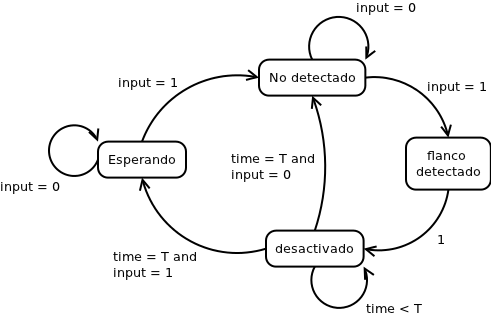
\includegraphics[width=0.5\textwidth]{edgeDetectorDebounceFSM.png}
	\caption{Máquina de estados}\label{fig:edgeDetectorDebounceFSM}
\end{figure}

El detector de flancos con antirrebote es un detector de flancos estándar al que se le ha añadido un temporizador que lo desactiva durante un cierto periodo de tiempo tras detectar un flanco, para evitar las oscilaciones producidas por los rebotes de los pulsadores.

Su diseño está basado en una máquina de estados simple (figura \ref{fig:edgeDetectorDebounceFSM}) que consta de cuatro estados: ``no detectado'', ``flanco detectado'', ``desactivado'' y ``esperando''. La máquina empieza en el estado ``no detectado'', y permanece en él mientras la entrada valga 0. Cuando recibe un 1, pasa al estado ``flanco detectado'', y la salida se pone a 1 hasta el siguiente flanco de reloj, en el cual pasa al estado
``desactivado'', poniendo la salida a 0. Mientras la máquina se encuentra en este estado, un temporizador cuenta el tiempo transcurrido, y bloquea el paso al estado siguiente. Cuando el tiempo deseado, en nuestro caso 100 ms,  ha transcurrido, la máquina de estados pasará al estado ``no detectado'' si la entrada es 0 o a ``esperando' si es 1. La máquina pasará entonces al estado de ``no detectado'' cuando reciba un 0 lógico.

\paragraph{Banco de pruebas}
Para probar este bloque se diseñó un banco de pruebas que simulaba una entrada ruidosa, con varias oscilaciones entre nivel alto y bajo, de forma que se comprobase que el detector sólo se activaba una vez tras el flanco, con una duración de un periodo de reloj.
\subsection{Jugador (Player)}
\label{player}

\begin{figure}[H]
	\centering
	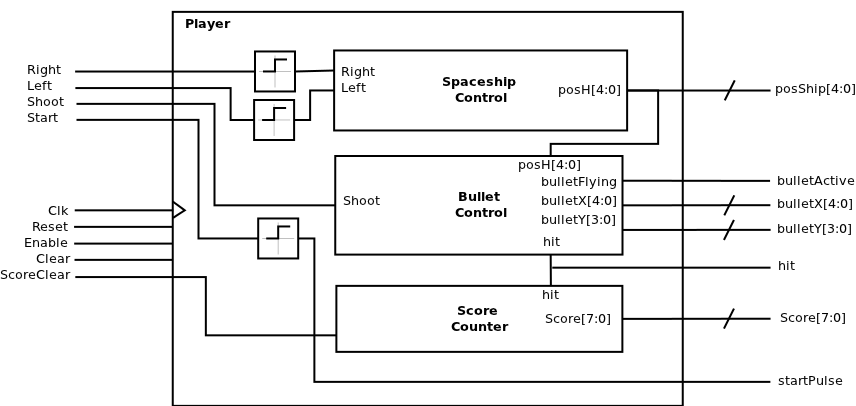
\includegraphics[width=0.6\textwidth]{player_block.png}
	\caption{Diagrama de bloques del Jugador (player) }\label{fig:playerBlock}
\end{figure}

Con el fin de agrupar todas las funciones de un jugador para mayor claridad, hemos creado un bloque Jugador (Player) que incluye toda la funcionalidad del jugador, de forma que además podemos instanciar varios jugadores de forma sencilla. Esto ha facilitado el añadir un segundo jugador a nuestro juego, simplemente instanciando este bloque 2 veces.

El bloque Jugador (figura \ref{fig:playerBlock}) incluye: tres detectores de flancos con antirrebote para las señales de movimiento a izquierda y derecha y de inicio, un control de la nave, un control del disparo y un contador para la puntuación.

También posee una serie de señales de control del bloque: Reset asíncrono, Clear síncrono ( pone todo a su estado inicial excepto la puntuación), un Clear síncrono para la puntuación y una entrada Enable para su habilitación, que afecta a todos los bloques excepto al detector de flancos de inicio, que siempre está activo.

La implementación en VHDL simplemente instancia los bloques necesarios y realiza las conexiones entre ellos. El contador de la puntación, sin embargo, se ha implementado como un proceso, que incrementa una unidad el contador cada vez que le llega una señal de marciano alcanzado por un disparo (hit).


\subsection{Control de los invasores (Invaders)}
\label{invaders}

\begin{figure}[H]
	\centering
	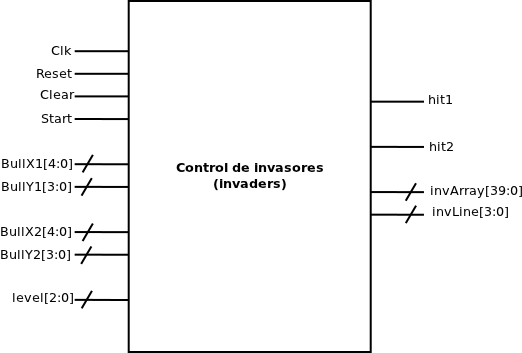
\includegraphics[width=0.4\textwidth]{invaders_block.png}
	\caption{Diagrama de bloques del Control de los invasores (Invaders) }\label{fig:invadersBlock}
\end{figure}

El bloque de control de los invasores se encarga tanto del movimiento de los invasores a lo largo de la pantalla, como de comprobar la posición del disparo y matar a los correspondientes marcianos. Para ello, además de las entradas de control típicas (Clk, Reset, Clear) posee 2 conjuntos de entradas que le proporcionan la posición y estado de cada una de las 2 balas del juego (una por cada jugador).

Para ello hemos definido una matriz constante que almacena la disposición inicial de los marcianos para cada uno de los 8 niveles implementados. Esta disposición se selecciona a través de la entrada ``level'', que indica el nivel actual.

Existen tres tipos de invasor, dependiendo del número de vidas que tengan (verde, 1 vida; amarillo, 2 vidas y blanco, 3 vidas) que se codifican usando 2 bits, siendo 00 un hueco sin marciano, 01 un marciano verde, 10 un marciano amarillo y 11 un marciano blanco, de 3 vidas. Estos marcianos se guardan en un vector de 40 elementos, 2 elementos por casilla de la pantalla en la que puede haber un marciano, que como se ha mencionado previamente, se selecciona dependiendo del nivel actual.

Este bloque también posee dos temporizadores que controlan la velocidad de avance de los invasores. Dependiendo del nivel se selecciona uno u otro, teniendo dos velocidades posibles (normal y rápida). Se seleccionó este diseño en lugar de un sólo temporizador con 8 velocidades (una por nivel) debido a que al haber aumentado la dificultad añadiendo marcianos más poderosos no tenía mucho sentido incrementarla aún más aumentando la velocidad en sólo 8 niveles, y había recursos suficientes en la FPGA como para poner dos teporizadores, cuyo diseño ya estaba realizado en prácticas anteriores, en lugar de uno nuevo con varias comprobaciones de cuenta.

La implementación en VHDL posee una señal ``start'', que sirve de señal de disparo, cambiando el estado de un biestable interno ``moving'' que indica al bloque que los marcianos han comenzado a moverse. Una vez en movimiento, cada pulso de reloj (en el que el temporizador lo permita), el vector de marcianos sufre un desplazamiento de 2 posiciones hacia la derecha. Si una de las 2 últimas posiciones del vector contiene un 1, es decir, si un marciano ha llegado al final de la línea, la posición en el eje Y se incrementa una unidad, y se invierte el sentido del desplazamiento. Este proceso se repite hasta que todos los marcianos hayan muerto, o hayan llegado a la última posición.

Por último se comprueba si el disparo coincide con la posición de alguno de los marcianos, y si es así, decrementa la vida del marciano en 1 unidad (un marciano blanco pasaría a ser amarillo, uno amarillo a ser verde, y uno verde moriría) y envía un pulso a través de la señal ``hit1'' o ``hit2'', dependiendo de qué jugador haya alcanzado al marciano.
\section{Conclusión / Posibles mejoras}
%
\end{document}